\documentclass[10pt,conference,compsocconf]{IEEEtran}
\usepackage{hyperref}
\usepackage{graphicx}
\usepackage{xcolor}
\usepackage{blindtext, amsmath, comment, subfig}
\usepackage{grffile}
\usepackage{caption}
\usepackage[utf8]{inputenc}
\usepackage[backend=biber, style=ieee, sorting=none]{biblatex}
\addbibresource{references.bib}

\pagenumbering{X}
\title{CS-523 SecretStroll Report}
\author{Francesco Intoci, Elvric Trombert}
\date{Spring Semester 2020-2021}



\addtolength{\oddsidemargin}{-.21in}
\addtolength{\textwidth}{0.25in}
\addtolength{\topmargin}{-.15in}
\addtolength{\textheight}{.15in}

\begin{document}



\maketitle

\begin{abstract}
    This paper aims to describe our design choice for the "SecretStroll" LBS system, together with a Privacy Evaluation of the system itself.
\end{abstract}

\section{Introduction}
SecretStroll is a Location Based System (LBS), which aims to provide users with
information about Points of Interest (POI) near their location, satisfying
user-specified criteria.\newline
LBS are prone to be privacy-sensitive system: if not implemented following a
\textit{Privacy by Design} paradigm, they can leak many information about users,
such as their location and movement patterns, which can lead to more
privacy-disruptive attacks. For this reason, we designed SecretStroll
by identifying layers at which the system could potentially leak information and
implementing privacy-preserving mechanism to try mitigating such leaks. We also conducted a privacy evaluation of the system.\newline
\subsection{Attribute-based credential}
SecretStroll exploits an Attribute-based credential Protocol to authorize users
to fetch POIs of a given type, for which they must have subscribed to. The ABC protocol serves to purposes:
first, it allows the server to check whether a user request is valid, w.r.t the payment status of the
user for that service. Secondly, it guarantees anonymity to the users, since the server will not be able
to link a credential to a user after subsequent requests.
\subsection{(De)Anonymization of User Trajectories}
ABC alone are not enough in order to guarantee users privacy. In particular, if the server is
able to observe users metadata, such as their IP Address, the ABC scheme clearly looses its
\textit{unlinkability} property. We analyzed the consequences on users' privacy of attacks
mounted by an adversary with access to such metadata, and we evaluated a defence mechanism aimed to mitigate
such attacks.
\subsection{Fingerprinting attack on Tor}
SecretStroll exploits the Tor Network in order not to leak metadata at Network level. Nevertheless, we
evaluated the privacy offered by this solution. In particular, supposing that an adversary was able to
sniff the traffic between a client and the entry guard of Tor network, we mounted a \textit{web fingerprinting}
attack to try inferring the grid location of the user querying the service.
\section{Attribute-based credential}
For the implementation of the authorization through \textit{Attribute-based
credentials}, we have carefully followed the protocol described by
\textit{Pointcheval and Sanders} \cite{PS_signature}. Nevertheless, during the
development of the \textit{ABC} system, some design challenges needed to be
solve, and it is worth highlighting their solution:
\begin{itemize}
    \item \textbf{Server-Client agreement on the attribute domain}: as described
    in \cite{PS_signature}, before even starting the protocol, server and client
    must agree on the public parameters, including the number $L$ of possible
    attributes. Moreover, users should choose attributes (subscriptions) which
    are recognized by the server. To this end, we decided to embed the list of
    available subscriptions in the server public key. The 'attribute domain' is thus formed by the
    $L-2$ possible subscriptions, followed by the username and a client secret key.
    Clients are expected to choose their subscriptions from the provided set:
    failing to comply with the protocol on client side will result in the
    abortion by the server.
    \item \textbf{Attribute encoding}: once we designed the server-client
    agreement in such a way that each parameter of the public key was mapped to one attribute, we decided to encode
    attributes in the following way: if the user decides to subscribe to service
    $i$, then the exponent of public key parameter $i$ is a fixed prime number in $Z_p$ (where $p$ is the order of
    the prime groups defined in the paper): \texttt{SUBSCRIBED\_YES}. Conversely, any service to which the client does
    not subscribe, is encoded with a different fixed prime:
    \texttt{SUBSCRIBED\_NO}. The 'username' attribute is encoded through
    \texttt{int.from\_bytes(username.encode(), 'big')}. Client secret key is a random number in $Z_p$.
    \item \textbf{Fiat-Shamir Heuristic for Issuance Request}: Clients choose their \textit{user-defined} attributes,
    which in our implementation are the secret key and username, together with a
    blinding factor $t$. Note that the random blinding factor guarantees
    \textit{issuer unlinkability}. User commitment $C$ will thus be
    $g^{t}*Y_{L}^{client\_sk}$. Client will also produce a \textit{NIZKP} of his commitment. In order
    to generate the challenge in a non interactive way, we applied
    \textit{Fiat-Shamir Heuristic} to the \textit{sigma protocol} defined for
    the \textit{Pedersen's Commitment PK}: the provided
    challenge was the \textit{sha256} digest of the public parameters (the
    commitment $C$, the randomness $R$ of the proof, and the public key
    parameters used for exponentiation, $g$ and $Y_{L}^{client\_sk}$)
    \item \textbf{Fiat-Shamir Heuristic for linking Disclosure Proof to
    location}: \textit{Fiat Shamir Heuristic} plays also a crucial role when
    linking the \textit{Showing protocol} of the paper to a specific message
    (i.e client's current location). This prevents a malicious user
    eavesdropping communication to steal one user's credential in order to gain
    access to the service from its current location, different from the one of the user. In order to apply
    \textit{Fiat-Shamir Heuristic}, we modelled the \textit{Disclosure Proof} as
    a regular \textit{NIZKP} on Pedersen's Commitment, where generators belong
    to the $G_T$ group: \[PK\{(t,a_i), i \in H : C=e(\sigma_{1}^{`},
    \tilde{g})^t\prod_{i \in H}e(\tilde{Y}_{i}^{a_i},\tilde{g})\}\]
    Thus, the generators in the Proof of Knowledge are $e(\sigma_{1}^{`}, \tilde{g})$ and
    $e(\tilde{Y}_{i},\tilde{g})$. In order to link the location to the
    proof, we used a \textit{Schnorr's Signature}, producing the challenge as:
    \[c = sha256(R|C|public\_parameters|location)\]
    The server validations follows two steps: first, it checks it can recompute client's commitment via
    the \textit{bilinear} property of the pairing:
    \[C = e(\sigma_2^`,\tilde{g})\prod_{i \in
    D}e(\sigma_1^`,\tilde{Y}_i)^{-a_i}e(\sigma_1^`,\tilde{X})^{-1}\] Secondly,
    it checks the validity of the proof on client's commitment.
\end{itemize}
\subsection{Test}
In order to test the correctness of our \textit{ABC protocol}, we implemented a
simple test suite using \texttt{pytest} called \texttt{test\_abc.py}, involving
a correct run of the protocol and 4 runs where the client deviate from the
protocol in different ways:
\begin{itemize}
    \item \texttt{test\_registering\_invalid\_attributes}: client issues a
    request with an attribute which do not belong to the agreed domain.
    \item \texttt{test\_requesting\_service\_not\_subscribed}: client tries to
    request a service to which it did not subscribe. Implicitly, this will lead
    to a \textit{Disclosure Proof} which is not valid for the given credentials.
    \item \texttt{test\_invalid\_signature\_on\_message}: simulates a passive
    adversary who is able to eavesdrop communication between another user and
    the server, trying to ask for a given service, from its current location, by
    replaying the \textit{Disclosure Proof} sent by a client from a different
    location.
    \item \texttt{test\_invalid\_user\_commitment}: when creating the issue
    request, client presents a proof which is not valid for his commitment.
\end{itemize}

\subsection{Evaluation}
For the evaluation of the \textit{ABC protocol}, we analyzed how the
communication cost in terms of exchanged bytes, and the computational cost in
terms of runtime, variate in respect to the number of available subscriptions:
\begin{figure}[h!]
    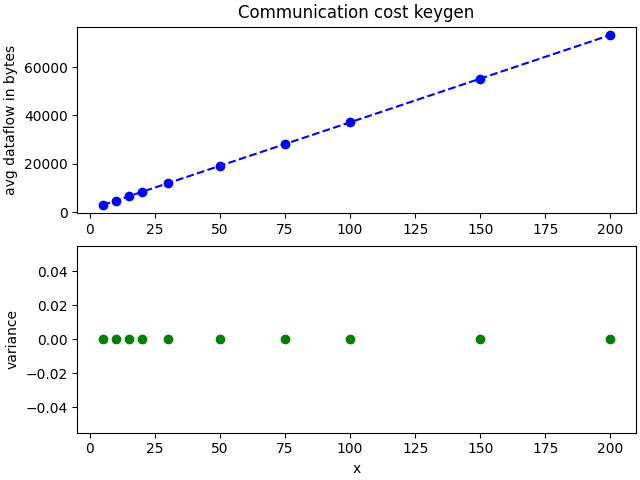
\includegraphics[width=0.4\linewidth]{../performance_analysis/dataflow_keygen.png}
    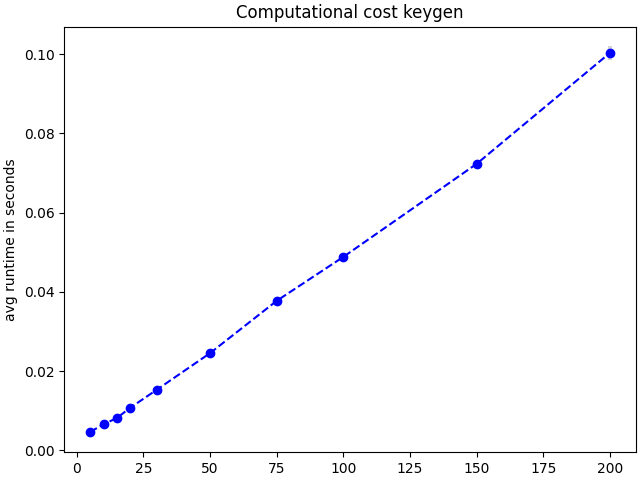
\includegraphics[width=0.4\linewidth]{../performance_analysis/runtime_keygen.png}
    \caption{Avg dataflow and runtime for the key generation step}
    \label{fig:keygen}
\end{figure}

\begin{figure}[h!]
    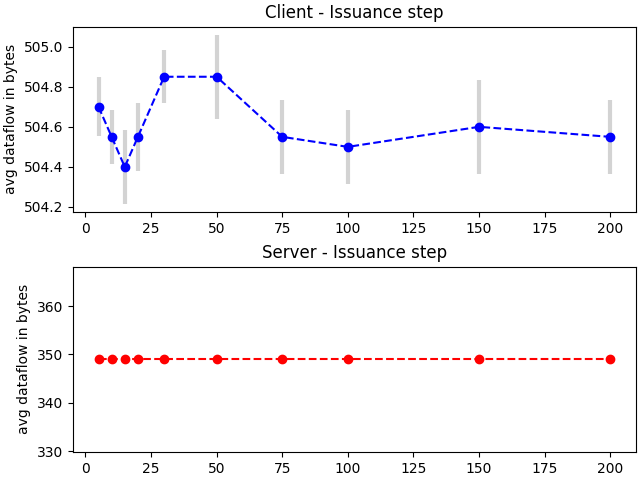
\includegraphics[width=0.4\linewidth]{../performance_analysis/dataflow_issuance.png}
    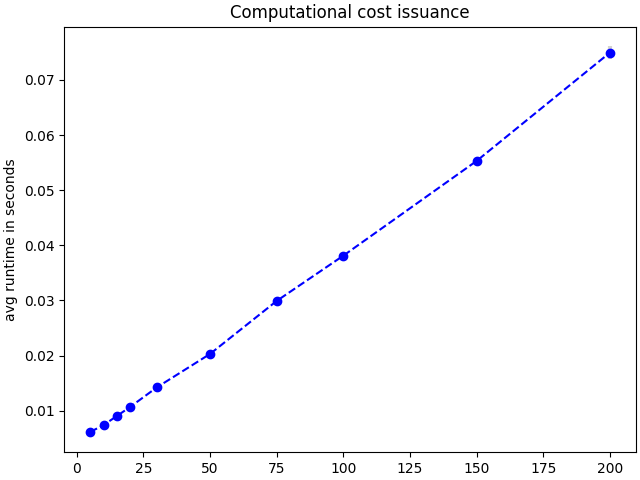
\includegraphics[width=0.4\linewidth]{../performance_analysis/runtime_issuance.png}
    \caption{Avg dataflow and runtime for the credential issuing}
    \label{fig:issuance}
\end{figure}


\begin{figure}[h!]
    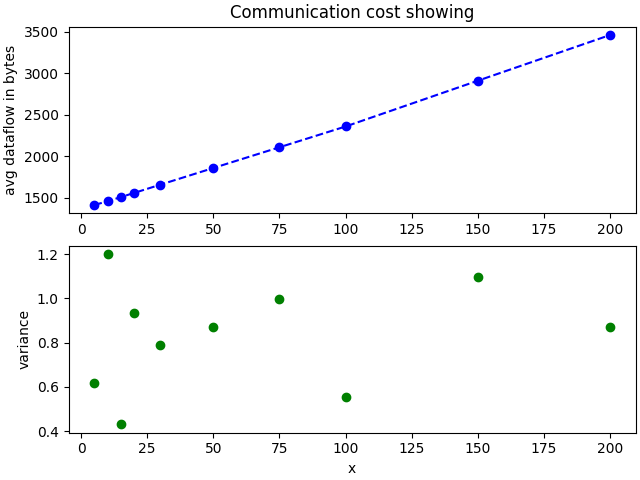
\includegraphics[width=0.4\linewidth]{../performance_analysis/dataflow_showing.png}
    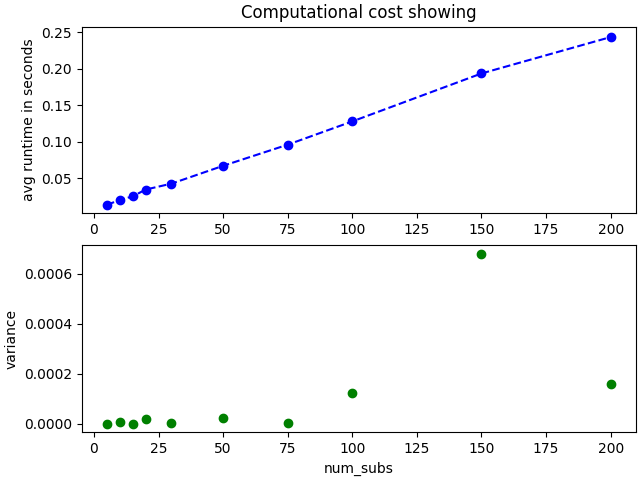
\includegraphics[width=0.4\linewidth]{../performance_analysis/runtime_showing.png}
    \caption{avg dataflow and runtime for client request}
    \label{fig:showing}
\end{figure}

\begin{figure}[h!]
    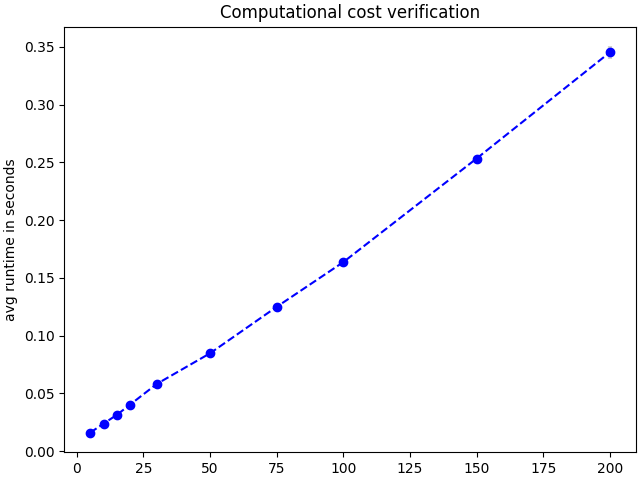
\includegraphics[width=0.4\linewidth]{../performance_analysis/runtime_verification}
    \caption{avg runtime for the credential verifications}
    \label{fig:verify}
\end{figure}


\section{(De)Anonymization of User Trajectories}

\subsection{Privacy Evaluation}
In this section, we performed a privacy evaluation on the network level of
SecretStroll.


\subsubsection{Identity Inference Attack}


\paragraph{Threat Model}
For this attack, we considered a \textbf{passive} adversary (i.e \textit{Honest
but Curious}). We modelled the adversary as \textbf{global} (i.e she has a full
view of the network used by the system, meaning that she can eavesdrop queries
made from whichever cell in SecretStroll grid. The adversarial view is
represented by \texttt{queries.csv} dataset). More specifically, the adversary
in this setting is SecretStroll \textbf{service provider}.\newline
We assumed the following background knowledge for the adversary: the adversary
knows a mapping between users' IP addresses and their name and surname.\newline
We assumed the adversary computational power to be bounded by Polynomial time.


\paragraph{Adversarial Goal}
The goal of the adversary is to infer users' \textbf{top-3 locations}, namely
their home location, their workplace location, and any particular place where
they spend their leisure time. By knowing such sensible information and
combining with her background knowledge, the adversary can uniquely identify
users.


\paragraph{Implementation Details}
\begin{itemize}
    \item \textbf{Feature Extraction}: the first step for performing the attack
    was a simple process of feature extraction. We added 4 new columns to the
    \textit{queries.csv} dataset from the \textit{timestamp} column:
    \textit{cell_id} column, \textit{hour} column (hour granularity),
    \textit{day} column (from day $1$ to $20$) and \textit{daytime}
    column (it represents when the query was made during the day. For example, a query launched
    at 10 a.m was labelled as "Morning").
    \item \textbf{Trajectory Analysis}: the second step was to
    analyze the "quality" of the provided data: generally, when performing
    inference on users home or workplace location, the common assumption is that
    users follow a habitual pattern. Before
    mounting the attack, we decided to test this assumption. We collected, for
    each IP address, their daily trajectory (as a time-ordered sequence of
    latitude and longitude coordinates). We then computed the distance matrix
    between each pair of daily trajectories using \textit{Frechet Distance}. The
    results showed that, for each users, trajectories were very similar.
    Furthermore we could assess that \textit{Frechet Distance} represented a
    meaningful metric, since for each user we could witness a larger distance
    between trajectories collected during week days and trajectories collected
    during weekends (as expected by the different pattern of average people
    during work days compared to their pattern during days off).


    \begin{figure}[h!]
        \centering
        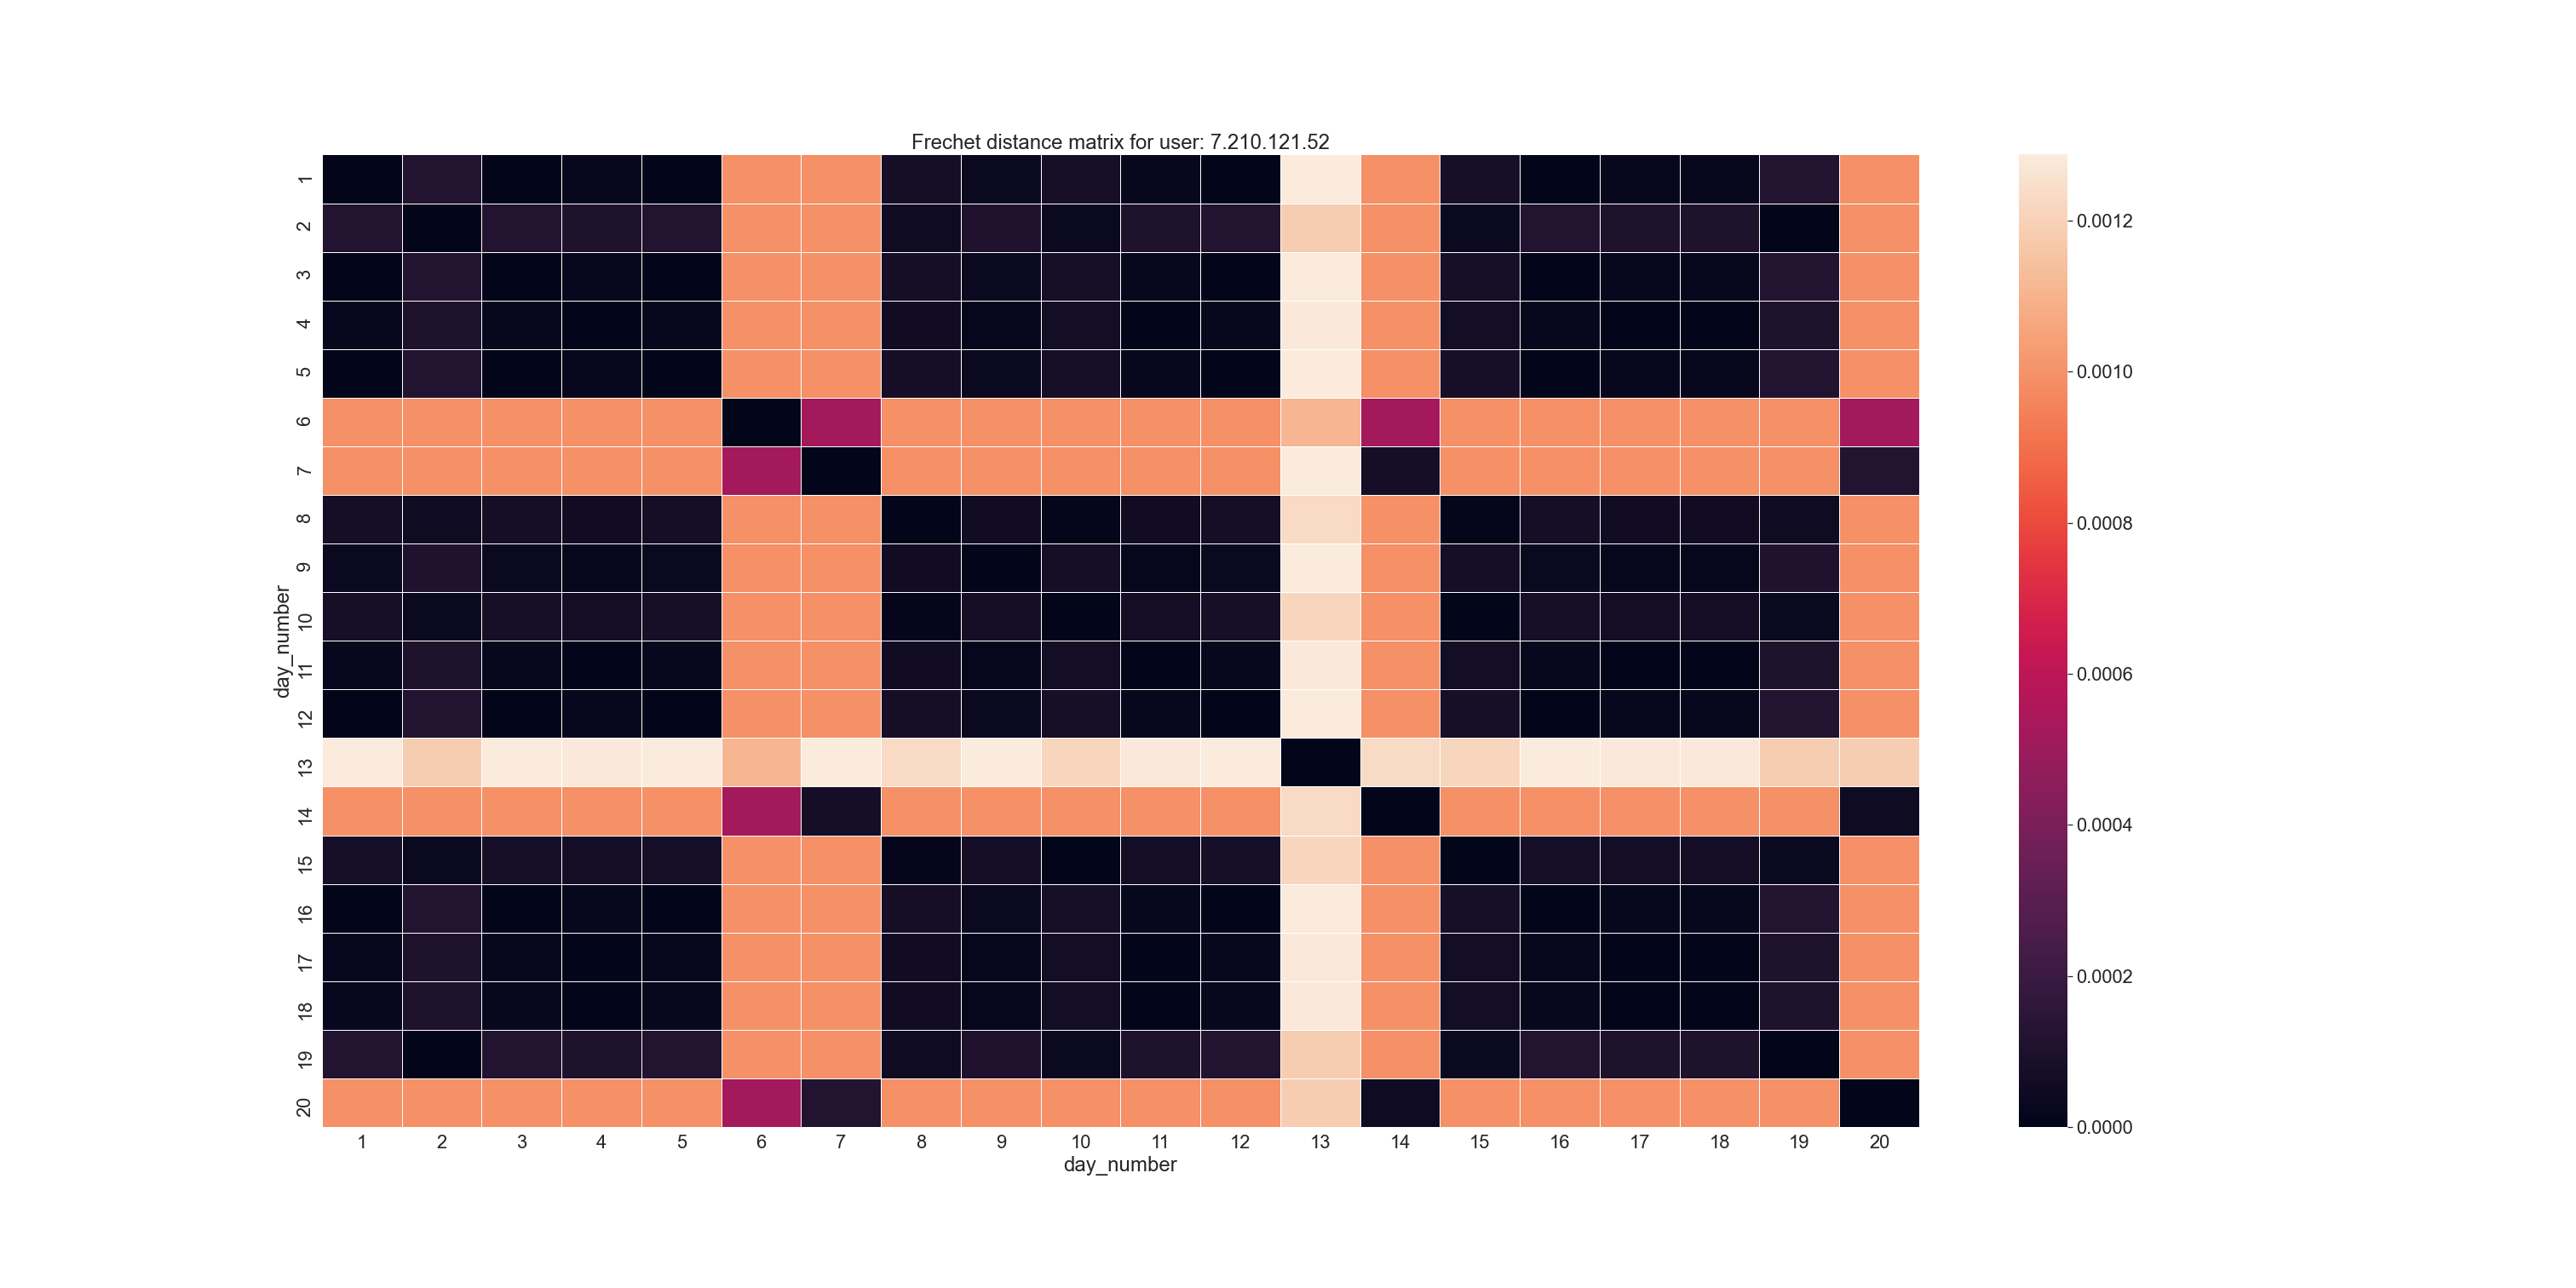
\includegraphics[width=0.5\linewidth]{../privacy_evaluation/daily_trajectories/7.210.121.52-matrix.png}
        \caption{Distance Matrix of one user}
        \label{fig:matrix}
    \end{figure}


    \item \textbf{Location clustering}: After validating the data, we proceeded
    to mount the attack. We first grouped the daytimes we defined in three groups ("home", "work", "leisure") accordingly to where a user was likely to be in that moment. For example, the group \textit{daytime home},
    was comprehensive of daytimes "Early" and "Night". Then, for
    each user, for each daytime group, we
    extracted latitudes and longitudes of locations. Then, we fed the
    coordinates to the \textbf{DBSCAN} algorithm. After
    the clusters were formed, we filtered out the noise and computed
    the centroid of the biggest cluster. Results are provided in the \texttt{top\_locations.csv} file. It is
    worth noticing that, for a few users, there were not enough queries during
    the "Evening" to infer something about their "leisure time" top location.
\end{itemize}

\subsubsection{De-anonimization of trajectories trough Co-Location}

\paragraph{Reference}
The idea for the attack was taken by reading https://ieeexplore.ieee.org/document/8228621.
\paragraph{Threat Model}
For this attack, similarly to the previous one, we considered the adversary to
be again the \textbf{service provider}(thus again
\textbf{passive} and \textbf{global}).
As far as her background knowledge is concerned, we assumed that the adversary
knows the identity of a subset of users. With respect to her capabilities, we assumed that
the adversary has access to a side channel of information about users, more
concretely to users' public profiles on social networks. Our additional assumption is that all targeted users on the OSN made queries to SecretStroll.

\paragraph{Adversarial Goal}
The goal of the adversary is to infer the identity of users for which she does
not know a name-IP address mapping. In order to do so, the adversary looks for
similarity, on daily basis, on users trajectories, in order to exploit the
co-location information provided by users' OSN profiles. Suppose that IP address "IP A" belongs to a user for
whom the adversary knows the identity: Alice. After running the attack, the
adversary knows that, on day 6, Alice's trajectory was very similar to the one
of user with ip address "IP B". The adversary exploits her side channel
and discovers, visiting Alice profile, that, on day 6, Alice spent the
day with her friend Bob. The adversary can thus infer with good probability that
user having "IP B" is Bob.

\paragraph{Implementation Details}
We adopted an approach very similar to step 2 of the previous attack. For each
day, we collected each user trajectory. For users whose trajectories were made
up of fewer points than the longest trajectory of the day, the last known
position was used as padding. We then computed the distance matrix between
trajectories, using again \textit{Frechet Distance}. Finally, we used
\textbf{DSBSCAN} algorithm in order to find clusters within the trajectories. We
reported, for each day where a cluster of size greater than one was found, the
users whose trajectories belonged to the same cluster, and the day. The results
are provided in the \texttt{users\_trajectories\_similarities.csv} file.


\subsection{Defences}
In order to protect users privacy against the attacks we described in section
\textit{A}, we designed the following \textit{Location Privacy Preserving
Mechanism}. When accessing the application at client side, users will select a
parameter $p$, to which we refer as \textit{obfuscation probability}. When
performing a query to the service, the application will retain the current user
location with probability $1-p$. With probability $p$, the client will choose a
random location in the current cell in which the user is located or one of the
neighbouring cell (depending if the cell is at one corner of the grid, the
number of available neighbours will vary between $2$ and $4$).
\subsubsection{Adversarial Models}
The LPPM we designed is aimed to protect users against attacks $1$ and $2$ in
section \textit{A}, by introducing noise in the localization mechanism used by
the system. Thus, the adversarial models we took into account are the ones we
described in the first two aforementioned attacks. Clearly, the mechanism is ineffective
against the adversarial model described in attack $3$.
\subsubsection{Assumptions}
When evaluating our mechanism, the following assumptions were made:
\begin{itemize}
    \item \textbf{Ground Truth}: Since we were not provided with the ground
    truth about users in the dataset (i.e the real location of their house and
    workplace), we assumed the results obtained by the adversary of attack $1$
    without the mechanism in place as ground truth.
    \item \textbf{Strategic Adversary}: In our evaluation, we considered a
    strategic adversary, i.e we assumed that the adversary knew the details
    about the mechanism and that she could consequently mount the best attack
    possible. Nevertheless, we assumed that the adversary did not know the value
    of $p$ chosen each time by the client.\newline
    Consequently, the adversary we used for our evaluation was able to
    dynamically adapt is algorithm. More details about this in the following
    section about the evaluation.
\end{itemize}
\subsubsection{Privacy Gain Evaluation}
For the evaluation of the Privacy Gain introduced by our mechanism, we simulated
the same scenario of attack $1$. The following changes were made:
\begin{itemize}
    \item \textbf{Client}: we modified the queries dataset applying the LPPM. In
    each test, a different value of $p$ was used.
    \item \textbf{Adversary}: the adversary used the same algorithm described in
    attack $1$, as we believed that the algorithm could perform well for the
    adversary even in presence of noise (DBSCAN is capable of labelling points
    as noise). Nevertheless, taking into account that the adversary is
    strategic, we modified the algorithm to adapt to the amount of noise
    detected by DBSCAN. If the clustering algorithm returned at least two points
    labelled as "not noisy", then the algorithm proceeded as described. If no
    "not noisy" points were found, the adversary used the centroid of the
    "noise" cluster as prediction (since the noise added by the mechanism is
    uniformly added along all directions, there is a probability that by
    averaging out the noise the adversary can find a good enough prediction).
\end{itemize}
As Privacy metric, we used a metric applied in the literature \cite{Shokri}, the
\textbf{Expected Adversarial Error}, i.e the distortion introduced by the
mechanism in the outcome of the adversary inference in respect to her inference
without the mechanism:
\[Privacy = \frac{\sum_{i=1}^{i=n_{users}}haversine(x, \tilde{x})}{n_{users}}\] where $x$ is the
original prediction and $\tilde{x}$ is the distorted one. The evaluation took
into account both predictions for home and workplace locations. As distance
metric, we used the \textit{haversine} distance between the predicted points (as
latitude-longitude pairs), in kilometers.
    \begin{figure}[h!]
        \centering
        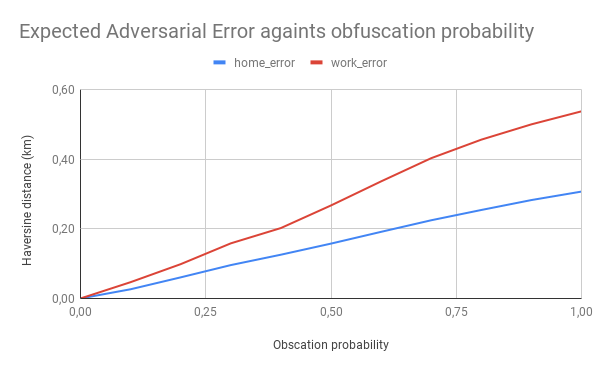
\includegraphics[width=0.5\linewidth]{../privacy_evaluation/adv_error.png}
        \caption{Privacy gain evaluation}
    \end{figure}
\subsubsection{Utility Loss Evaluation}
For the evaluation of the Utility Loss which the mechanism eventually adds, we
reported the percentage of queries for which the mechanism produced a change in
the cell identifier in which the user appeared located, against the parameter
$p$.
\begin{figure}[h!]
    \centering
    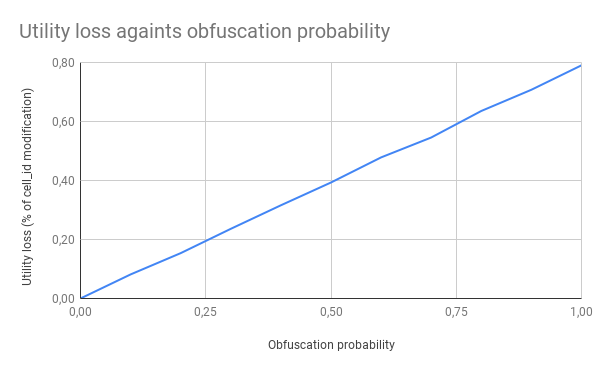
\includegraphics[width=0.5\linewidth]{../privacy_evaluation/utility_loss.png}
    \caption{Utility Loss evaluation}
\end{figure}
\subsubsection{Utility-Privacy Trade-off}
As showed in the previous plots, the mechanism parameter $p$ is directly
proportional (linearly) to the Privacy Gain of the users as well to the Utility
Loss introduced in the application.
\section{Cell Fingerprinting via Network Traffic Analysis}

\subsection{Implementation details}
\subsubsection{Trace collection}
//TO DO
\subsubsection{Filtering}
Before proceeding with feature extraction, we decided to apply two filters to the captured traces:
\begin{itemize}
    \item \textbf{Less than 609 B}: we analyzed the traffic between client and server, using Tor, when the client did not perform any request. We found out that packets were sent. Nevertheless, these packets were all below the size of $609B$. In particular, we have seen that at TLS level the frame size was $543 B$ , that appears to be standard for TLS application data sent inside single TOR cells.  For this reasons, we filtered out packets below this threshold when evesdropping client requests.
    \item \textbf{Removed TCP ACKs}: Following an approach found in literature \cite{web_fingerprinting}, we decided to remove TCP ACKs sent by the server since they did not carry any payload.
\end{itemize}
\subsubsection{Feature Extraction}
In order to select a suitable set of features for the classification task, we tried to follow the features presented in the lecture notes, as well as in literature \cite{web_fingerprinting}:
\begin{itemize}
    \item 1 - Total number of packets.
    \item 2 - Number of incoming packets from server.
    \item 3 - Ratio between number of incoming packets and total number of packets.
    \item 4 - Ratio between number of packets sent by client and total.
    \item 5 - Total number of bytes exchanged in KB.
    \item 6 - Number of incoming bytes in KB.
    \item 7 - Ratio between incoming bytes and total bytes.
    \item 8 - Ratio between bytes sent by client and total bytes.
    \item 9 - Average size of incoming packets in KB.
    \item 10 - Markers: how many time the direction of flow changes in the capture.
    \item 11 - 13 Top 3 Bursts size in KB.
    \item 14 - 16 Top 3 Bursts timestamp in seconds.
    \item 17 - 19 Top 3 Bursts sequence number in capture.
    \item 20 - 21 Percentage fluctuation in packet sizes, i.e ratio between first packet size and median packet size, and between median and last packet sizes.
    \item 22 Average time interval between incoming packets in nanoseconds.
\end{itemize}
\subsection{Evaluation}
In order to perform the multi-label classification, we trained a \textit{Random Forest Classifier} provided by the \texttt{sklearn} library. In order to evaluate the performance of the classifier, we used the Exact Match Ratio metric. As validation method, we used a 10-fold stratified cross validation, and repeated the evaluation 5 times.

\subsection{Discussion and Countermeasures}
The overall result of the model was very good, scoring an accuracy of $0.926$ with a standard deviation of $0.006$.
The attack achieved good results even with less traces, scoring around $0.82$ accuracy with $0.02$ standard deviation with just 30 samples per cell.
This very effective attack represents one of the limitation of Tor system. Nevertheless, it is possible to adopt some countermeasures in order to lower the success rate (i.e accuracy, in this case), of the attack. For example, one technique could be \textit{traffic morphing}. Since the classifier we built mainly relies on packets size and timing, \textit{SecretStroll} server could try to uniform data from all the cells, for example adding decoy POIs, in order to pad the response for every grid queried by the user such that they all have the same lenght. Furthermore, it could add some random delay between sending packets (at cost of latency), so to hide the peculiar timing for each cell response.



\printbibliography

\end{document}
